
\section{Two-Dimensional Collisions\footnote{
1990-93 Dept. of Physics and Astronomy, Dickinson College. Supported by FIPSE
(U.S. Dept. of Ed.) and NSF. Portions of this material may have been modified
locally and may not have been classroom tested at Dickinson College.
}}

\makelabheader %(Space for student name, etc., defined in master.tex or labmanual_formatting_commands.tex)

\bigskip
\textbf{Objectives} 

To test experimentally that the Law of Conservation of Momentum holds for two-dimensional
collisions.

\bigskip
\textbf{Apparatus}

\begin{itemize}[nosep]
\item A set of ball bearings, a protractor, a level, some carts, 
and a wooden board.
\item A video analysis system (\textit{Tracker}).
\end{itemize}

\bigskip
\textbf{2-D Collisions: Intelligent Guesses \& Observations }

Conservation of momentum can be used to solve a variety of collision and explosion
problems. So far we have only considered momentum conservation in one dimension,
but real collisions lead to motions in two and three dimensions. For example,
air molecules are continually colliding in space and bouncing off in different
directions. 

You probably know more about two-dimensional collisions than you think. Draw
on your prior experience with one-dimensional collisions to anticipate the outcome
of several two-dimensional collisions. Suppose you were a witness to several
accidents in which you closed your eyes at the moment of collision each time
two vehicles heading toward each other crashed. Even though you couldn't stand
to look, can you predict the outcome of the following accidents?

You see car A enter an intersection at the same time as car B coming from its
left enters the intersection. Car B is the same make and model as car A and
is traveling at the same speed. The two cars collide and bounce off one another.
What happens? Hint: You can use a symmetry argument, your intuition or a quick
analysis of 1-D results. For example, pick a coordinate system and think about
two separate accidents: the x accident in which car B is moving at speed \( v_{bx} \)
and car A is standing still, and the y accident in which car A is moving at
speed \( v_{ay} \) = \( v_{bx} \) and car B is standing still. 

%\vspace{0.5cm}
%{\par\centering 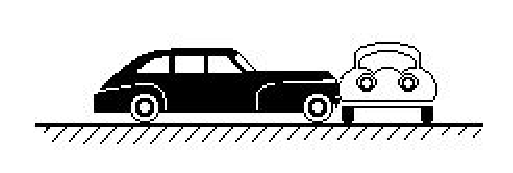
\includegraphics[scale=1.2]{twod_collisions/twod_collisions_fig1.eps} \par}
%\vspace{0.5cm}

The diagram below shows an aerial view of several possible two-dimensional accidents
that might occur. The first is a collision at right angles of two identical
cars.

%\vspace{0.3cm}
%{\par\centering 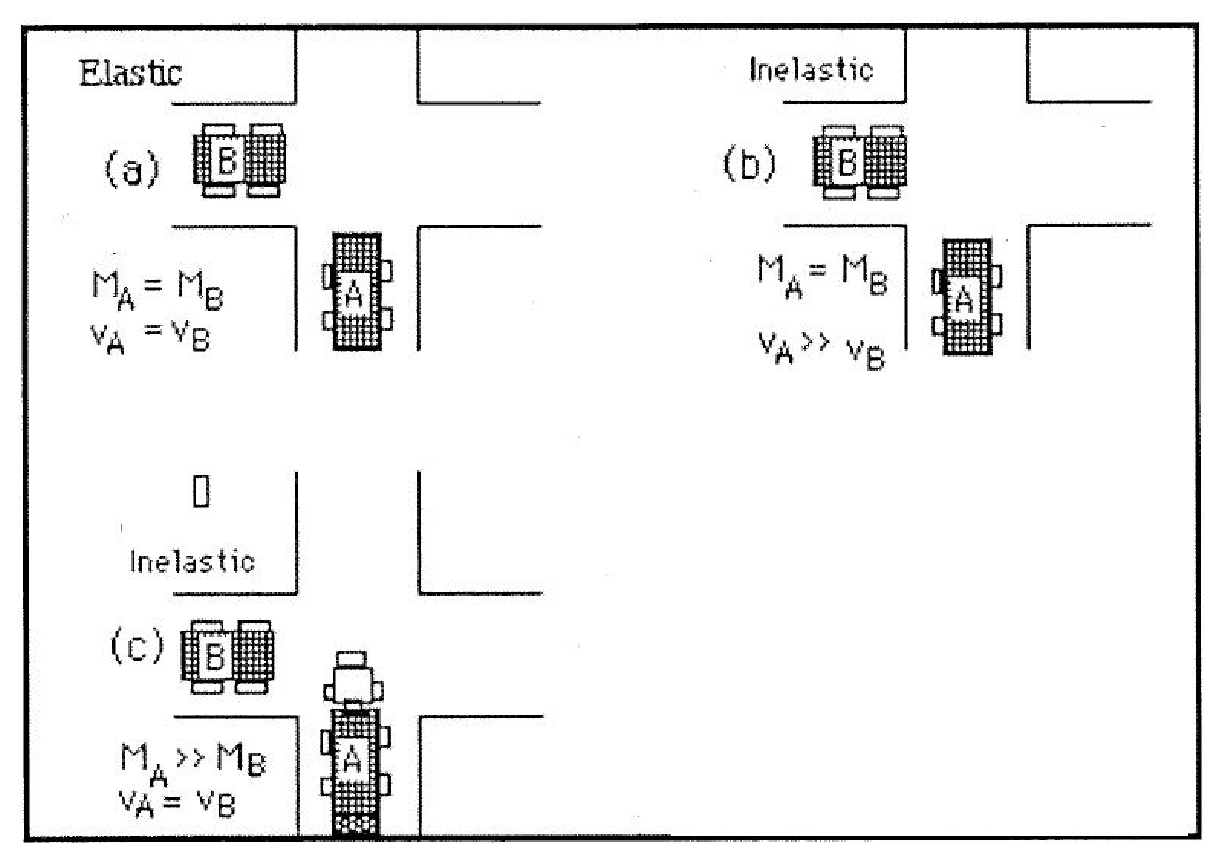
\includegraphics[width=4.8in,]{twod_collisions/twod_collisions_fig1s.eps} \par}
%\vspace{0.3cm}

\textbf{Activity 1: Qualitative 2-D Collisions }

(a) On the diagram below, draw a dotted line in the direction you think
two cars will move after an elastic collision between cars with equal masses and equal velocities.
Also explain your reasoning in the space below.

\hspace{0.3in}
\includegraphics{twod_collisions/two_equal_cars.eps}

\pagebreak[3]
(b) Draw a dotted line for the direction the cars might move after an inelastic collision if car A is traveling
at a speed much greater than that of car B. Explain your reasoning in the space
below. 

\hspace{0.3in}
\includegraphics{twod_collisions/two_cars_unequal_speeds.eps}

(c) If instead of a car, the vehicle A were a large truck traveling at the same
speed as car B, in what direction will the vehicles move? Draw the dotted lines.
Explain your reasoning in the space below.

\hspace{0.3in}
\includegraphics{twod_collisions/car_and_truck.eps}

%(d) Now suppose that the two vehicles are traveling at the same speed. If the
%two vehicles were to stick together; in what direction would they move after
%the collision, if they undergo a perfectly inelastic collision? Explain your
%reasoning in the space below.
%\vspace{20mm}

(d) Finally, set up these types of collisions. Observe each type of collision
several times. Draw solid lines in the diagram above for the results. How good
were your predictions? Explain your reasoning in the space below.
\answerspace{30mm}

(e) What rules have you devised to predict more or less what is going to happen
as the result of a two-dimensional collision?
\answerspace{15mm}

\pagebreak[3]
\textbf{Theory of 2D Momentum Conservation }

Since momentum is a vector, the Law of Conservation of Momentum in two dimensions
requires that if the vector conservation equation is broken into components
then the conservation law must also hold for each of the vector components.
Thus, if we consider the interaction of several objects, and if 
\[
\sum {\vec p}={{\vec p}_{1i}}+{{\vec p}_{2i}}+{{\vec p}_{3i}}+\ldots ={{\vec p}_{1f}}+{{\vec p}_{2f}}+{{\vec p}_{3f}}+\ldots =\mbox{a constant}\]
then
\[
\sum p_{x}=(p_{1i})_{x}+(p_{2i})_{x}+(p_{3i})_{x}+\ldots = (p_{1f})_{x}+(p_{2f})_{x}+(p_{3f})_{x}+\ldots =
\mbox{a constant}\]


and
\[
\sum p_{y}=(p_{1i})_{y}+(p_{2i})_{y}+(p_{3i})_{y}+\ldots = (p_{1f})_{y}+(p_{2f})_{y}+(p_{3f})_{y}+\ldots =
\mbox{a constant}\]


If a coordinate system is chosen and a given momentum vector makes an angle
\( \theta  \) with respect to the designated $x$-axis then the momentum vector
can be broken into components in the usual way:
\[
{\vec p}=p_{x}~\widehat{i}+p_{y}~\widehat{ j}=p\cos \theta~\widehat{ i}+
p\sin \theta~\widehat{ j}\]


%Let's consider an interaction in which a large mass collides with two smaller
%hard masses connected by a blob of clay. Assume that this interaction causes
%the bundle of masses to divide into three fragments as shown in the figure below.

%\vspace{0.3cm}
%{\par\centering 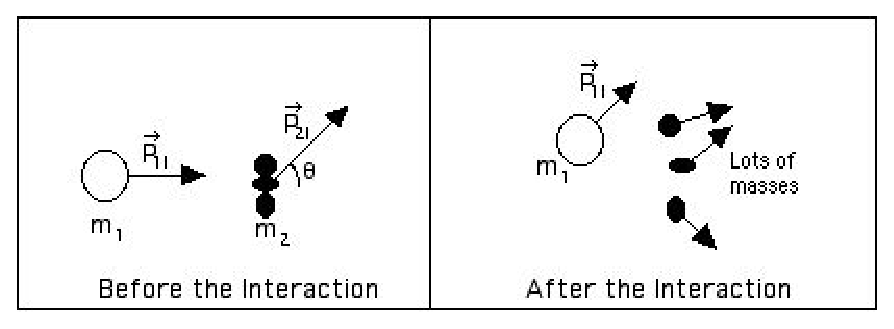
\includegraphics{twod_collisions/twod_collisions_fig3.eps} \par}
%\vspace{0.3cm}

%\textbf{Activity 2: Taking Components }

%(a) Consider mass \#1. Suppose \( m_{1}  = 2.0 \)kg and the speed \( v_{1i} 
%= 1.5 \) m/s. What is the initial x-component of momentum? The initial y-component
%of momentum? Show your calculations.
%\vspace{5mm}

%\( p_{1ix} \) = 
%\vspace{5mm}

%\( p_{1iy} \) = 
%\vspace{5mm}

%(b) Consider mass \#2. Suppose \( m_{2}  = 1.8 \) kg and the speed 
%\( v_{2i} 
%= 2.3 \) m/s. If \( \theta   = 40^{\circ } \), what is the initial x-component
%of momentum? The initial y-component of momentum? Show your calculations.
%\vspace{20mm}

\textbf{Is Momentum Conserved in Two Dimensions? }

During the last few sessions we have placed a lot of faith in the power of Newton's
second and third laws to predict that momentum is always conserved in collisions.
We have tested the conservation of momentum for one-dimensional collisions and
have shown mathematically and experimentally for one-dimensional collisions
that if momentum is conserved the center- of-mass of a system will move at a
constant velocity regardless of how many internal interactions take place. Now,
let's test whether a collision in an isolated two body system will conserve
momentum within the limits of experimental uncertainty. 

Consider two ball bearings that are free to move in two dimensions on a table.
We will record and analyze a video of the two bearings colliding. You can then
find the $x$- and $y$-components of the momentum for each bearing and test the 
conservation of momentum in a closed system. 

\textbf{Activity 2: Testing the Conservation of Momentum }

(a) Make a movie of two ball bearings colliding by following these steps. 

\begin{enumerate}
\item Turn the camera on and center the wooden board in the field of view. The camera
should be about 1 m above the center of the board where one bearing(the target)
will sit. The target bearing should be located straight down below the camera.
 Make sure the board is flat by using the small level available at each station. 
 Place a ruler somewhere
in the field of view where it won't interfere with the collision and parallel
to one edge of the field of view. This ruler will be user later to determine
the scale. 
\item Make a movie of one bearing (the projectile) rolling into the other, stationary
bearing (the target). See \textbf{Appendix \ref{tracker}: Video Analysis Using Tracker} 
for details on making the movie. Make the collision a glancing one so that the 
projectile is scattered to some large angle (otherwise, you will only test 
momentum conservation in one dimension).
\end{enumerate}
(b) Determine the position of each bearing (the target and the projectile) 
using \textit{Tracker}. In \textit{Tracker}, align one of the axes along the 
path of the incoming projectile. Track one object, then the other as functions 
of time. For each object you will have a table with three columns with the 
values of time, $x$ and $y$ positions of each object.
%To do this task follow the instructions in \textbf{Appendix
%\ref{videopoint}: Video Analysis} for creating, calibrating, and analyzing movie data. On each
%frame click once on the projectile bearing and once on the target. The data
%table should contain five columns with the values of time, x and y positions
%of the projectile, and x and y positions of the target. 
%When you calibrate the movie data, note the number of frames per second and 
%record the time interval between successive frames.
\vspace{5mm}

%\( \Delta  t\) = 
%\vspace{5mm}

(c) Record the masses of the two ball bearings.
\vspace{5mm}

\( m_{1} =\)  \hfill{}\( m_{2} =\)  \hfill{}
\vspace{5mm}

(d) Create graphs of $x$ \textit{vs.}~time and $y$ \textit{vs.}~time for each object.
\vspace{7mm}

%(e) Draw by eye a best-fit line through the points corresponding to the trajectory
%of the projectile before the collision. This line will become a new x-axis when
%you analyze the momentum components of the system. Draw best-fit lines through
%the points for both ball bearings after the collision. What are the angles of
%the paths of the target and projectile after the collision with respect to trajectory of the incoming projectile before the collision? 
%\vspace{10mm}

(e) Use the graphs to measure the distance each bearing covered before and after
the collision. What is the average velocity for each ball bearing before and
after the collision?
\vspace{7mm}

\( (v_{1i})_{x}= \) \hfill{}\( (v_{1i})_{y}= \)  \hfill{}
\vspace{7mm}

\( (v_{2i})_{x} =\)  \hfill{}\( (v_{2i})_{y}= \)  \hfill{}
\vspace{7mm}

\( (v_{1f})_{x} =\)  \hfill{}\( (v_{1f})_{y}= \)  \hfill{}
\vspace{7mm}

\((v_{2f})_{x} =\)  \hfill{}\( (v_{2f})_{y}= \)  \hfill{}
\vspace{7mm}


(f) What are the momentum components for each ball bearing before and after
the collision?
\vspace{7mm}

\( (p_{1i})_{x}= \) \hfill{}\( (p_{1i})_{y}= \)  \hfill{}
\vspace{7mm}

\( (p_{2i})_{x} =\)  \hfill{}\( (p_{2i})_{y}= \)  \hfill{}
\vspace{7mm}

\( (p_{1f})_{x} =\)  \hfill{}\( (p_{1f})_{y}= \)  \hfill{}
\vspace{7mm}

\((p_{2f})_{x} =\)  \hfill{}\( (p_{2f})_{y}= \)  \hfill{}
\vspace{7mm}


(g) What is the total momentum of the system in each direction before the 
collision?
\vspace{7mm}

\( (p_{i})_{x} =\)  \hfill{}\( (p_{i})_{y}= \) \hfill{} 
\vspace{7mm}

(h) What is the total momentum of the system in each direction after the 
collision?
\vspace{7mm}

\( (p_{f})_{x} =\)  \hfill{}\( (p_{f})_{y}= \) \hfill{} 
\vspace{7mm}

\newpage

(i) Calculate the difference between the initial, total momentum in the $x$ direction and the final, total momentum in the $x$ direction from your data ($(p_{f})_{x} - (p_{i})_{x}$).
Calculate the difference between the initial, total momentum in the $y$ direction and the final, total momentum in the $y$ direction from your data ($(p_{f})_{y} - (p_{i})_{y}$).
Record your results here.
\vspace{50mm}

(j) What would you expect for the difference between the initial and final total momentum in the $x$ and $y$ directions? Calculate the percent difference in each direction.
%Do the data from the class support this expectation? 
%Use the averages and standard deviations for the class to quantitatively answer this question.
\vspace{50mm}

(k) Does total momentum seem to be conserved?
